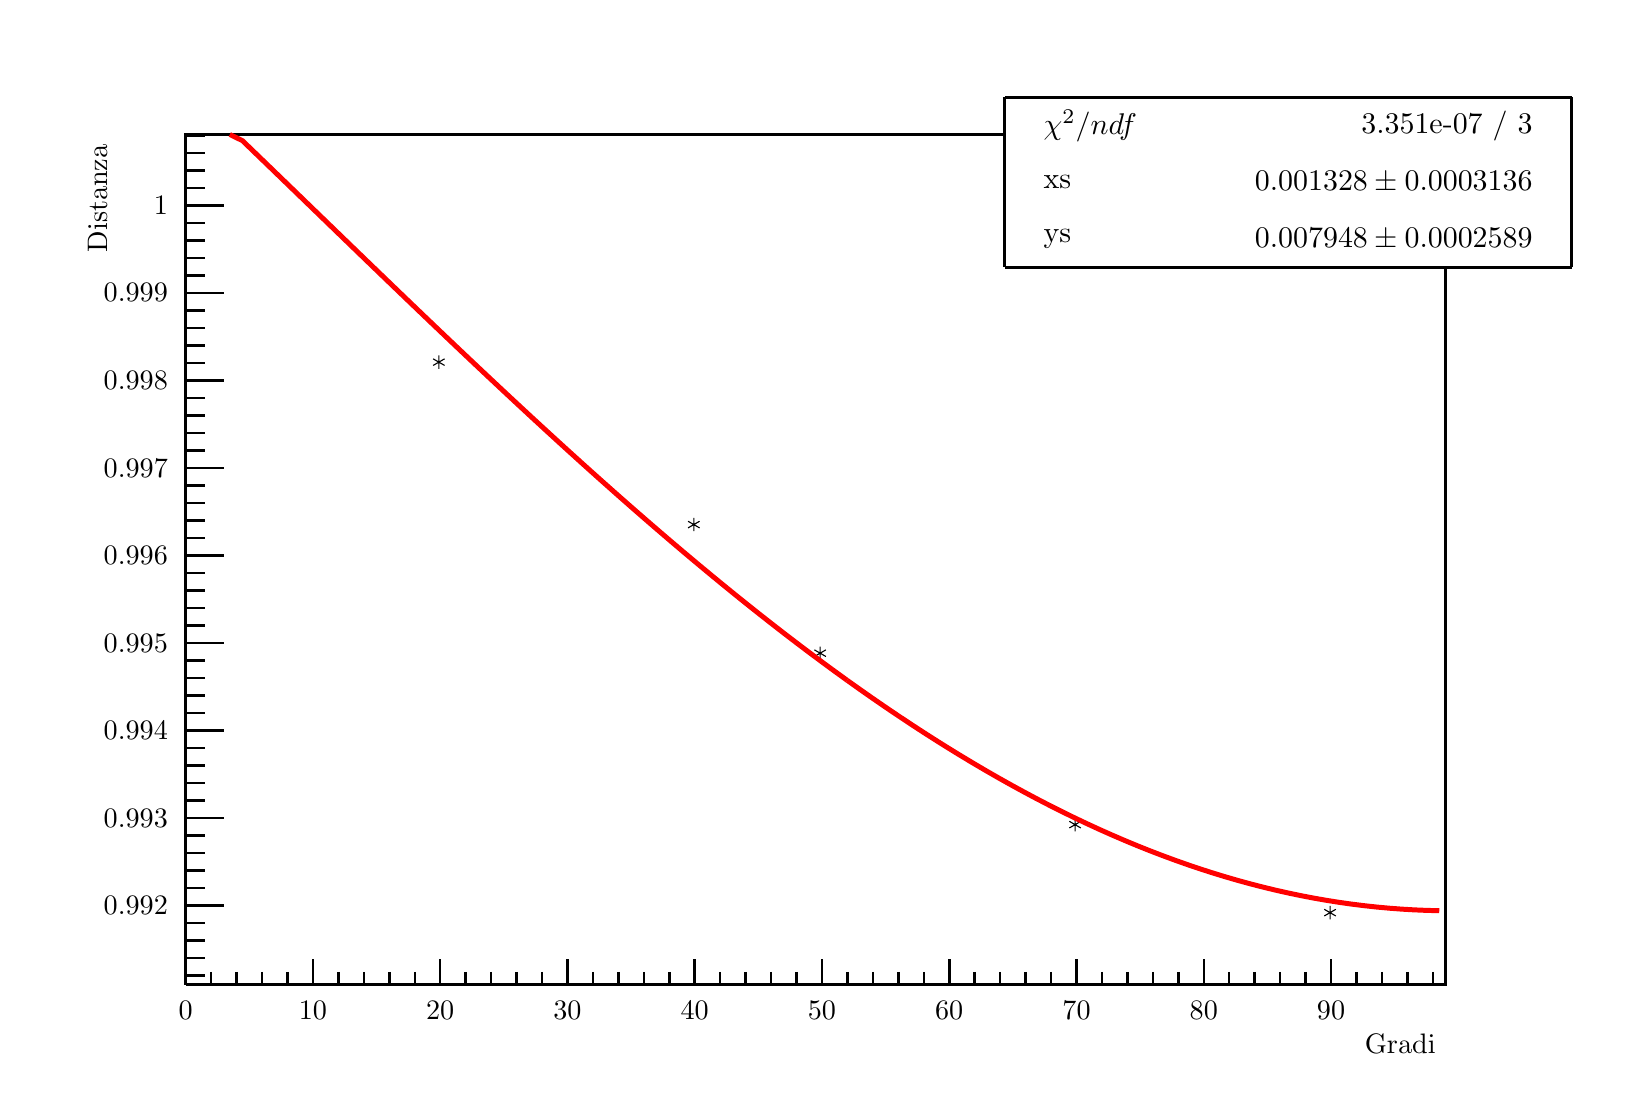
\begin{tikzpicture}
\pgfdeclareplotmark{cross} {
\pgfpathmoveto{\pgfpoint{-0.3\pgfplotmarksize}{\pgfplotmarksize}}
\pgfpathlineto{\pgfpoint{+0.3\pgfplotmarksize}{\pgfplotmarksize}}
\pgfpathlineto{\pgfpoint{+0.3\pgfplotmarksize}{0.3\pgfplotmarksize}}
\pgfpathlineto{\pgfpoint{+1\pgfplotmarksize}{0.3\pgfplotmarksize}}
\pgfpathlineto{\pgfpoint{+1\pgfplotmarksize}{-0.3\pgfplotmarksize}}
\pgfpathlineto{\pgfpoint{+0.3\pgfplotmarksize}{-0.3\pgfplotmarksize}}
\pgfpathlineto{\pgfpoint{+0.3\pgfplotmarksize}{-1.\pgfplotmarksize}}
\pgfpathlineto{\pgfpoint{-0.3\pgfplotmarksize}{-1.\pgfplotmarksize}}
\pgfpathlineto{\pgfpoint{-0.3\pgfplotmarksize}{-0.3\pgfplotmarksize}}
\pgfpathlineto{\pgfpoint{-1.\pgfplotmarksize}{-0.3\pgfplotmarksize}}
\pgfpathlineto{\pgfpoint{-1.\pgfplotmarksize}{0.3\pgfplotmarksize}}
\pgfpathlineto{\pgfpoint{-0.3\pgfplotmarksize}{0.3\pgfplotmarksize}}
\pgfpathclose
\pgfusepathqstroke
}
\pgfdeclareplotmark{cross*} {
\pgfpathmoveto{\pgfpoint{-0.3\pgfplotmarksize}{\pgfplotmarksize}}
\pgfpathlineto{\pgfpoint{+0.3\pgfplotmarksize}{\pgfplotmarksize}}
\pgfpathlineto{\pgfpoint{+0.3\pgfplotmarksize}{0.3\pgfplotmarksize}}
\pgfpathlineto{\pgfpoint{+1\pgfplotmarksize}{0.3\pgfplotmarksize}}
\pgfpathlineto{\pgfpoint{+1\pgfplotmarksize}{-0.3\pgfplotmarksize}}
\pgfpathlineto{\pgfpoint{+0.3\pgfplotmarksize}{-0.3\pgfplotmarksize}}
\pgfpathlineto{\pgfpoint{+0.3\pgfplotmarksize}{-1.\pgfplotmarksize}}
\pgfpathlineto{\pgfpoint{-0.3\pgfplotmarksize}{-1.\pgfplotmarksize}}
\pgfpathlineto{\pgfpoint{-0.3\pgfplotmarksize}{-0.3\pgfplotmarksize}}
\pgfpathlineto{\pgfpoint{-1.\pgfplotmarksize}{-0.3\pgfplotmarksize}}
\pgfpathlineto{\pgfpoint{-1.\pgfplotmarksize}{0.3\pgfplotmarksize}}
\pgfpathlineto{\pgfpoint{-0.3\pgfplotmarksize}{0.3\pgfplotmarksize}}
\pgfpathclose
\pgfusepathqfillstroke
}
\pgfdeclareplotmark{newstar} {
\pgfpathmoveto{\pgfqpoint{0pt}{\pgfplotmarksize}}
\pgfpathlineto{\pgfqpointpolar{44}{0.5\pgfplotmarksize}}
\pgfpathlineto{\pgfqpointpolar{18}{\pgfplotmarksize}}
\pgfpathlineto{\pgfqpointpolar{-20}{0.5\pgfplotmarksize}}
\pgfpathlineto{\pgfqpointpolar{-54}{\pgfplotmarksize}}
\pgfpathlineto{\pgfqpointpolar{-90}{0.5\pgfplotmarksize}}
\pgfpathlineto{\pgfqpointpolar{234}{\pgfplotmarksize}}
\pgfpathlineto{\pgfqpointpolar{198}{0.5\pgfplotmarksize}}
\pgfpathlineto{\pgfqpointpolar{162}{\pgfplotmarksize}}
\pgfpathlineto{\pgfqpointpolar{134}{0.5\pgfplotmarksize}}
\pgfpathclose
\pgfusepathqstroke
}
\pgfdeclareplotmark{newstar*} {
\pgfpathmoveto{\pgfqpoint{0pt}{\pgfplotmarksize}}
\pgfpathlineto{\pgfqpointpolar{44}{0.5\pgfplotmarksize}}
\pgfpathlineto{\pgfqpointpolar{18}{\pgfplotmarksize}}
\pgfpathlineto{\pgfqpointpolar{-20}{0.5\pgfplotmarksize}}
\pgfpathlineto{\pgfqpointpolar{-54}{\pgfplotmarksize}}
\pgfpathlineto{\pgfqpointpolar{-90}{0.5\pgfplotmarksize}}
\pgfpathlineto{\pgfqpointpolar{234}{\pgfplotmarksize}}
\pgfpathlineto{\pgfqpointpolar{198}{0.5\pgfplotmarksize}}
\pgfpathlineto{\pgfqpointpolar{162}{\pgfplotmarksize}}
\pgfpathlineto{\pgfqpointpolar{134}{0.5\pgfplotmarksize}}
\pgfpathclose
\pgfusepathqfillstroke
}
\definecolor{c}{rgb}{1,1,1};
\draw [color=c, fill=c] (0,0) rectangle (20,13.4957);
\draw [color=c, fill=c] (2,1.34957) rectangle (18,12.1461);
\definecolor{c}{rgb}{0,0,0};
\draw [c,line width=0.9] (2,1.34957) -- (2,12.1461) -- (18,12.1461) -- (18,1.34957) -- (2,1.34957);
\definecolor{c}{rgb}{1,1,1};
\draw [color=c, fill=c] (2,1.34957) rectangle (18,12.1461);
\definecolor{c}{rgb}{0,0,0};
\draw [c,line width=0.9] (2,1.34957) -- (2,12.1461) -- (18,12.1461) -- (18,1.34957) -- (2,1.34957);
\draw [c,line width=0.9] (2,1.34957) -- (18,1.34957);
\draw [anchor= east] (18,0.593811) node[scale=1.01821, color=c, rotate=0]{Gradi};
\draw [c,line width=0.9] (2,1.67347) -- (2,1.34957);
\draw [c,line width=0.9] (2.32323,1.51152) -- (2.32323,1.34957);
\draw [c,line width=0.9] (2.64646,1.51152) -- (2.64646,1.34957);
\draw [c,line width=0.9] (2.9697,1.51152) -- (2.9697,1.34957);
\draw [c,line width=0.9] (3.29293,1.51152) -- (3.29293,1.34957);
\draw [c,line width=0.9] (3.61616,1.67347) -- (3.61616,1.34957);
\draw [c,line width=0.9] (3.93939,1.51152) -- (3.93939,1.34957);
\draw [c,line width=0.9] (4.26263,1.51152) -- (4.26263,1.34957);
\draw [c,line width=0.9] (4.58586,1.51152) -- (4.58586,1.34957);
\draw [c,line width=0.9] (4.90909,1.51152) -- (4.90909,1.34957);
\draw [c,line width=0.9] (5.23232,1.67347) -- (5.23232,1.34957);
\draw [c,line width=0.9] (5.55556,1.51152) -- (5.55556,1.34957);
\draw [c,line width=0.9] (5.87879,1.51152) -- (5.87879,1.34957);
\draw [c,line width=0.9] (6.20202,1.51152) -- (6.20202,1.34957);
\draw [c,line width=0.9] (6.52525,1.51152) -- (6.52525,1.34957);
\draw [c,line width=0.9] (6.84848,1.67347) -- (6.84848,1.34957);
\draw [c,line width=0.9] (7.17172,1.51152) -- (7.17172,1.34957);
\draw [c,line width=0.9] (7.49495,1.51152) -- (7.49495,1.34957);
\draw [c,line width=0.9] (7.81818,1.51152) -- (7.81818,1.34957);
\draw [c,line width=0.9] (8.14141,1.51152) -- (8.14141,1.34957);
\draw [c,line width=0.9] (8.46465,1.67347) -- (8.46465,1.34957);
\draw [c,line width=0.9] (8.78788,1.51152) -- (8.78788,1.34957);
\draw [c,line width=0.9] (9.11111,1.51152) -- (9.11111,1.34957);
\draw [c,line width=0.9] (9.43434,1.51152) -- (9.43434,1.34957);
\draw [c,line width=0.9] (9.75758,1.51152) -- (9.75758,1.34957);
\draw [c,line width=0.9] (10.0808,1.67347) -- (10.0808,1.34957);
\draw [c,line width=0.9] (10.404,1.51152) -- (10.404,1.34957);
\draw [c,line width=0.9] (10.7273,1.51152) -- (10.7273,1.34957);
\draw [c,line width=0.9] (11.0505,1.51152) -- (11.0505,1.34957);
\draw [c,line width=0.9] (11.3737,1.51152) -- (11.3737,1.34957);
\draw [c,line width=0.9] (11.697,1.67347) -- (11.697,1.34957);
\draw [c,line width=0.9] (12.0202,1.51152) -- (12.0202,1.34957);
\draw [c,line width=0.9] (12.3434,1.51152) -- (12.3434,1.34957);
\draw [c,line width=0.9] (12.6667,1.51152) -- (12.6667,1.34957);
\draw [c,line width=0.9] (12.9899,1.51152) -- (12.9899,1.34957);
\draw [c,line width=0.9] (13.3131,1.67347) -- (13.3131,1.34957);
\draw [c,line width=0.9] (13.6364,1.51152) -- (13.6364,1.34957);
\draw [c,line width=0.9] (13.9596,1.51152) -- (13.9596,1.34957);
\draw [c,line width=0.9] (14.2828,1.51152) -- (14.2828,1.34957);
\draw [c,line width=0.9] (14.6061,1.51152) -- (14.6061,1.34957);
\draw [c,line width=0.9] (14.9293,1.67347) -- (14.9293,1.34957);
\draw [c,line width=0.9] (15.2525,1.51152) -- (15.2525,1.34957);
\draw [c,line width=0.9] (15.5758,1.51152) -- (15.5758,1.34957);
\draw [c,line width=0.9] (15.899,1.51152) -- (15.899,1.34957);
\draw [c,line width=0.9] (16.2222,1.51152) -- (16.2222,1.34957);
\draw [c,line width=0.9] (16.5455,1.67347) -- (16.5455,1.34957);
\draw [c,line width=0.9] (16.5455,1.67347) -- (16.5455,1.34957);
\draw [c,line width=0.9] (16.8687,1.51152) -- (16.8687,1.34957);
\draw [c,line width=0.9] (17.1919,1.51152) -- (17.1919,1.34957);
\draw [c,line width=0.9] (17.5152,1.51152) -- (17.5152,1.34957);
\draw [c,line width=0.9] (17.8384,1.51152) -- (17.8384,1.34957);
\draw [anchor=base] (2,0.904212) node[scale=1.01821, color=c, rotate=0]{0};
\draw [anchor=base] (3.61616,0.904212) node[scale=1.01821, color=c, rotate=0]{10};
\draw [anchor=base] (5.23232,0.904212) node[scale=1.01821, color=c, rotate=0]{20};
\draw [anchor=base] (6.84848,0.904212) node[scale=1.01821, color=c, rotate=0]{30};
\draw [anchor=base] (8.46465,0.904212) node[scale=1.01821, color=c, rotate=0]{40};
\draw [anchor=base] (10.0808,0.904212) node[scale=1.01821, color=c, rotate=0]{50};
\draw [anchor=base] (11.697,0.904212) node[scale=1.01821, color=c, rotate=0]{60};
\draw [anchor=base] (13.3131,0.904212) node[scale=1.01821, color=c, rotate=0]{70};
\draw [anchor=base] (14.9293,0.904212) node[scale=1.01821, color=c, rotate=0]{80};
\draw [anchor=base] (16.5455,0.904212) node[scale=1.01821, color=c, rotate=0]{90};
\draw [c,line width=0.9] (2,1.34957) -- (2,12.1461);
\draw [anchor= east] (0.88,12.1461) node[scale=1.01821, color=c, rotate=90]{Distanza};
\draw [c,line width=0.9] (2.48,2.3521) -- (2,2.3521);
\draw [c,line width=0.9] (2.24,2.57446) -- (2,2.57446);
\draw [c,line width=0.9] (2.24,2.79682) -- (2,2.79682);
\draw [c,line width=0.9] (2.24,3.01918) -- (2,3.01918);
\draw [c,line width=0.9] (2.24,3.24153) -- (2,3.24153);
\draw [c,line width=0.9] (2.48,3.46389) -- (2,3.46389);
\draw [c,line width=0.9] (2.24,3.68625) -- (2,3.68625);
\draw [c,line width=0.9] (2.24,3.90861) -- (2,3.90861);
\draw [c,line width=0.9] (2.24,4.13097) -- (2,4.13097);
\draw [c,line width=0.9] (2.24,4.35332) -- (2,4.35332);
\draw [c,line width=0.9] (2.48,4.57568) -- (2,4.57568);
\draw [c,line width=0.9] (2.24,4.79804) -- (2,4.79804);
\draw [c,line width=0.9] (2.24,5.0204) -- (2,5.0204);
\draw [c,line width=0.9] (2.24,5.24276) -- (2,5.24276);
\draw [c,line width=0.9] (2.24,5.46511) -- (2,5.46511);
\draw [c,line width=0.9] (2.48,5.68747) -- (2,5.68747);
\draw [c,line width=0.9] (2.24,5.90983) -- (2,5.90983);
\draw [c,line width=0.9] (2.24,6.13219) -- (2,6.13219);
\draw [c,line width=0.9] (2.24,6.35454) -- (2,6.35454);
\draw [c,line width=0.9] (2.24,6.5769) -- (2,6.5769);
\draw [c,line width=0.9] (2.48,6.79926) -- (2,6.79926);
\draw [c,line width=0.9] (2.24,7.02162) -- (2,7.02162);
\draw [c,line width=0.9] (2.24,7.24398) -- (2,7.24398);
\draw [c,line width=0.9] (2.24,7.46633) -- (2,7.46633);
\draw [c,line width=0.9] (2.24,7.68869) -- (2,7.68869);
\draw [c,line width=0.9] (2.48,7.91105) -- (2,7.91105);
\draw [c,line width=0.9] (2.24,8.13341) -- (2,8.13341);
\draw [c,line width=0.9] (2.24,8.35577) -- (2,8.35577);
\draw [c,line width=0.9] (2.24,8.57812) -- (2,8.57812);
\draw [c,line width=0.9] (2.24,8.80048) -- (2,8.80048);
\draw [c,line width=0.9] (2.48,9.02284) -- (2,9.02284);
\draw [c,line width=0.9] (2.24,9.2452) -- (2,9.2452);
\draw [c,line width=0.9] (2.24,9.46756) -- (2,9.46756);
\draw [c,line width=0.9] (2.24,9.68991) -- (2,9.68991);
\draw [c,line width=0.9] (2.24,9.91227) -- (2,9.91227);
\draw [c,line width=0.9] (2.48,10.1346) -- (2,10.1346);
\draw [c,line width=0.9] (2.24,10.357) -- (2,10.357);
\draw [c,line width=0.9] (2.24,10.5793) -- (2,10.5793);
\draw [c,line width=0.9] (2.24,10.8017) -- (2,10.8017);
\draw [c,line width=0.9] (2.24,11.0241) -- (2,11.0241);
\draw [c,line width=0.9] (2.48,11.2464) -- (2,11.2464);
\draw [c,line width=0.9] (2.48,2.3521) -- (2,2.3521);
\draw [c,line width=0.9] (2.24,2.12975) -- (2,2.12975);
\draw [c,line width=0.9] (2.24,1.90739) -- (2,1.90739);
\draw [c,line width=0.9] (2.24,1.68503) -- (2,1.68503);
\draw [c,line width=0.9] (2.24,1.46267) -- (2,1.46267);
\draw [c,line width=0.9] (2.48,11.2464) -- (2,11.2464);
\draw [c,line width=0.9] (2.24,11.4688) -- (2,11.4688);
\draw [c,line width=0.9] (2.24,11.6911) -- (2,11.6911);
\draw [c,line width=0.9] (2.24,11.9135) -- (2,11.9135);
\draw [c,line width=0.9] (2.24,12.1358) -- (2,12.1358);
\draw [anchor= east] (1.9,2.3521) node[scale=1.01821, color=c, rotate=0]{0.992};
\draw [anchor= east] (1.9,3.46389) node[scale=1.01821, color=c, rotate=0]{0.993};
\draw [anchor= east] (1.9,4.57568) node[scale=1.01821, color=c, rotate=0]{0.994};
\draw [anchor= east] (1.9,5.68747) node[scale=1.01821, color=c, rotate=0]{0.995};
\draw [anchor= east] (1.9,6.79926) node[scale=1.01821, color=c, rotate=0]{0.996};
\draw [anchor= east] (1.9,7.91105) node[scale=1.01821, color=c, rotate=0]{0.997};
\draw [anchor= east] (1.9,9.02284) node[scale=1.01821, color=c, rotate=0]{0.998};
\draw [anchor= east] (1.9,10.1346) node[scale=1.01821, color=c, rotate=0]{0.999};
\draw [anchor= east] (1.9,11.2464) node[scale=1.01821, color=c, rotate=0]{1};
\definecolor{c}{rgb}{1,1,1};
\draw [color=c, fill=c] (12.4,10.4592) rectangle (19.6,12.6185);
\definecolor{c}{rgb}{0,0,0};
\draw [c,line width=0.9] (12.4,10.4592) -- (18,10.4592);
\draw [c,line width=0.9] (12.4,12.1461) -- (12.4,10.4592);
\draw [anchor= west] (12.76,12.2586) node[scale=1.08185, color=c, rotate=0]{$\chi^{2} / ndf $};
\draw [anchor= east] (19.24,12.2586) node[scale=1.08185, color=c, rotate=0]{ 3.351e-07 / 3};
\draw [anchor= west] (12.76,11.5388) node[scale=1.08185, color=c, rotate=0]{xs       };
\draw [anchor= east] (19.24,11.5388) node[scale=1.08185, color=c, rotate=0]{$ 0.001328 \pm 0.0003136$};
\draw [anchor= west] (12.76,10.8191) node[scale=1.08185, color=c, rotate=0]{ys       };
\draw [anchor= east] (19.24,10.8191) node[scale=1.08185, color=c, rotate=0]{$ 0.007948 \pm 0.0002589$};
\foreach \P in {(5.2149,9.25501), (8.45272,7.19198), (10.0573,5.55874), (13.2951,3.38109), (16.533,2.26361)}{\draw[mark options={color=c,fill=c},mark size=2.402402pt,mark=asterisk] plot coordinates {\P};}
\definecolor{c}{rgb}{1,0,0};
\draw [c,line width=1.8] (2.56,12.1461) -- (2.72,12.068) -- (2.88,11.9138) -- (3.04,11.7594) -- (3.2,11.6048) -- (3.36,11.4501) -- (3.52,11.2953) -- (3.68,11.1405) -- (3.84,10.9857) -- (4,10.831) -- (4.16,10.6763) -- (4.32,10.5219) -- (4.48,10.3677)
 -- (4.64,10.2137) -- (4.8,10.06) -- (4.96,9.90663) -- (5.12,9.75367) -- (5.28,9.60115) -- (5.44,9.44911) -- (5.6,9.29759) -- (5.76,9.14665) -- (5.92,8.99633) -- (6.08,8.84667) -- (6.24,8.69771) -- (6.4,8.54951) -- (6.56,8.40211) -- (6.72,8.25555) --
 (6.88,8.10987) -- (7.04,7.96513) -- (7.2,7.82136) -- (7.36,7.6786) -- (7.52,7.5369) -- (7.68,7.39631) -- (7.84,7.25686) -- (8,7.11859) -- (8.16,6.98156) -- (8.32,6.84579) -- (8.48,6.71134) -- (8.64,6.57823) -- (8.8,6.44652) -- (8.96,6.31624) --
 (9.12,6.18743) -- (9.28,6.06013) -- (9.44,5.93438) -- (9.6,5.81022) -- (9.76,5.68767) -- (9.92,5.56679) -- (10.08,5.44761) -- (10.24,5.33016) -- (10.4,5.21449);
\draw [c,line width=1.8] (10.4,5.21449) -- (10.56,5.10061) -- (10.72,4.98858) -- (10.88,4.87842) -- (11.04,4.77016) -- (11.2,4.66385) -- (11.36,4.5595) -- (11.52,4.45716) -- (11.68,4.35686) -- (11.84,4.25862) -- (12,4.16247) -- (12.16,4.06845) --
 (12.32,3.97659) -- (12.48,3.8869) -- (12.64,3.79942) -- (12.8,3.71418) -- (12.96,3.63119) -- (13.12,3.5505) -- (13.28,3.47211) -- (13.44,3.39606) -- (13.6,3.32237) -- (13.76,3.25106) -- (13.92,3.18214) -- (14.08,3.11566) -- (14.24,3.05161) --
 (14.4,2.99003) -- (14.56,2.93093) -- (14.72,2.87433) -- (14.88,2.82025) -- (15.04,2.7687) -- (15.2,2.7197) -- (15.36,2.67326) -- (15.52,2.6294) -- (15.68,2.58814) -- (15.84,2.54948) -- (16,2.51343) -- (16.16,2.48002) -- (16.32,2.44924) --
 (16.48,2.4211) -- (16.64,2.39562) -- (16.8,2.37281) -- (16.96,2.35267) -- (17.12,2.3352) -- (17.28,2.32041) -- (17.44,2.30831) -- (17.6,2.2989) -- (17.76,2.29219) -- (17.92,2.28817);
\definecolor{c}{rgb}{1,1,1};
\draw [color=c, fill=c] (12.4,10.4592) rectangle (19.6,12.6185);
\definecolor{c}{rgb}{0,0,0};
\draw [c,line width=0.9] (12.4,10.4592) -- (19.6,10.4592);
\draw [c,line width=0.9] (19.6,10.4592) -- (19.6,12.6185);
\draw [c,line width=0.9] (19.6,12.6185) -- (12.4,12.6185);
\draw [c,line width=0.9] (12.4,12.6185) -- (12.4,10.4592);
\draw [anchor= west] (12.76,12.2586) node[scale=1.08185, color=c, rotate=0]{$\chi^{2} / ndf $};
\draw [anchor= east] (19.24,12.2586) node[scale=1.08185, color=c, rotate=0]{ 3.351e-07 / 3};
\draw [anchor= west] (12.76,11.5388) node[scale=1.08185, color=c, rotate=0]{xs       };
\draw [anchor= east] (19.24,11.5388) node[scale=1.08185, color=c, rotate=0]{$ 0.001328 \pm 0.0003136$};
\draw [anchor= west] (12.76,10.8191) node[scale=1.08185, color=c, rotate=0]{ys       };
\draw [anchor= east] (19.24,10.8191) node[scale=1.08185, color=c, rotate=0]{$ 0.007948 \pm 0.0002589$};
\end{tikzpicture}
